\documentclass{article}
\usepackage{tikz}
\usepackage{booktabs}

\title{Apuntes de L\'{o}gica Digital}
\date{2023-05-08}
\author{Daniel Araya Rom\'{a}n}

\begin{document}
\maketitle
\newpage

\section*{1. Sistemas Binarios}

\paragraph*{}
\normalsize

\subsection*{1.1 Sistemas Digitales}

En los sistemas digitales electr\'{o}nicos actuales,
las se\~{n}ales emplean s\'{o}lo dos valores discretos
$\rightarrow binarios$. Un d\'{i}gito binario, llamado
\textbf{bit}, que puede tomar los valores 0 y 1.
Un sistema digital es una interconexi\'{o}n de m\'{o}dulos
digitales. Para entender como funciona cada m\'{o}dulo digital,
se necesiatan conocimientos b\'{a}sicos de circuitos digitales
y de su funci\'{o}n l\'{o}gica.

Un lenguaje importante para el dise\~{n}o digital es el \textbf{(HDL,
Hardware Description Language)}. Sirve para simular sistemas digitales
y verificar su funcionamiento antes de crearlos en hardware.
\medskip

\begin{center}
    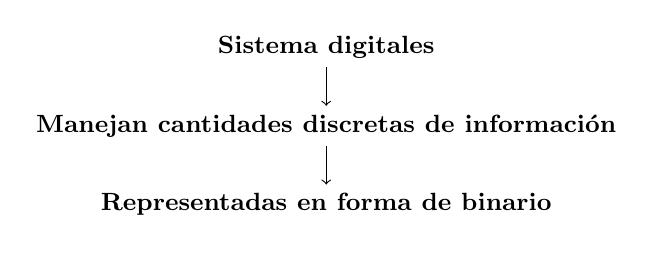
\begin{tikzpicture} 
        \small
        \node (a) at (0,0) {\textbf{Sistema digitales}};
        \node (b) at (0,-1) {\textbf{Manejan cantidades discretas de informaci\'{o}n}};
        \node (c) at (0,-2) {\textbf{Representadas en forma de binario}};
        \draw[->] (a) -- (b);
        \draw[->] (b) -- (c);
    \end{tikzpicture}
\end{center}
\medskip

\subsection*{1.2 N\'{u}meros Binarios}

\paragraph*{}
\normalsize

El n\'{u}mero decimal 7392, contiene potencias de 10 que est\'{a}n
impl\'{i}citas en la posici\'{o}n de los coeficientes, e.g:
\medskip

\begin{center}
    $7 \times 10^3 + 3 \times 10^2 + 9 \times 10^1 + 2 \times 10^0$
\end{center}

Un n\'{u}mero con punto decimal se representa con una serie de 
coeficientes, as\'{i}:

\begin{center}
    \large
    $a_5a_4a_3a_2a_1a_0 \cdot a_{-1}a_{-2}a_{-3}$
\end{center}

los coeficientes $a_j$ son cualesquiera de los 10 d\'{i}gitos (0...9);
el valor del sub\'{i}ndice $j$ indica la posici\'{o}n, y la potencia de
10 que se deber\'{a} multplicar ese coeficiente. De modo que:

\begin{center}
    $10^5a_5 + 10^4a_4 + 10^3a_3 + 10^2a_2 + 10^1a_1 + 10^0a_0
     + 10^-1a_{-1} + 10^-2a_{-2} + 10^-3a_{-3}$
\end{center}

El sistema binario es distinto al decimal, sus coeficientes solo pueden
tener 2 valores, 0 o 1. Cada coeficiente $a_j$ se multiplica por $2^j$.
11010.11 es 26.75 en decimal, porque:

\begin{center}
    $1 \times 2^4 + 1 \times 2^3 + 0 \times 2^2 + 1 \times 2^1 + 0 \times 2^0
     + 1 \times 2^{-1} + 1 \times 2^{-2} = 26.75$
\end{center}

En general, un n\'{u}mero expresado en un sistema de base \textbf{r} consiste
en coeficientes que se multiplican por potencias de \textbf{r}:

\begin{center}
    $a_n \cdot r^n + a_{n-1} \cdot r^{n-1} +...+ a_2 \cdot r^2 + a_1 \cdot r 
     + a_0 + a_{-1} \cdot r^{-1} + a_{-2} \cdot r^{-2} +...+ a_{-m} \cdot r^{-m}$
\end{center}

\subsection*{1.4 N\'{u}meros Octales y Hexadecimales}

Las conversiones entre binario, octal y hexadecimal son importantes en las 
computadoras digitales. Puesto que $2^3 = 8$ y $2^4 = 16$, cada d\'{i}gito
octal corresponde a \textbf{tres} d\'{i}gitos binarios, y cada d\'{i}gito
hexadecimal corresponde a \textbf{cuatro} d\'{i}gitos binarios.

$Binario \rightarrow octal$: agrupando los d\'{i}gitos binarios de 3 en 3,
de derecha a izquierda, y reemplazando cada grupo por su equivalente octal.
\begin{center}
    \large
    $(10\,110\,001\,101\,011 \cdot 111\,100\,000\,110)_2 = (26153.7406)_8$
\end{center}

$Binario \rightarrow hexadecimal$: agrupando los d\'{i}gitos binarios de 4 en 4,
de derecha a izquierda, y reemplazando cada grupo por su equivalente hexadecimal.
\begin{center}
    \large
    $(10\,1100\,0110\,1011 \cdot 1111\,0010)_2 = (2C6B.F2)_{16}$
\end{center}

Cuando se habla de binario es m\'{a}s deseable expresarlo en t\'{e}rminos de
n\'{u}meros octales o hexadecimales, porque son m\'{a}s compactos y f\'{a}ciles
de leer. As\'{i} $(111\,111\,111\,111)_2$ este n\'{u}mero en binario de 12 bits,
se puede escribir como $(7777)_8$ en octal o $(FFF)_{16}$ en hexadecimal.

\medskip

\begin{table}[h]
    \centering
    \begin{tabular}{cccc}
        \toprule
        Decimal & Binary & Octal & Hexadecimal \\
        (base 10) & (base 2) & (base 8) & (base 16) \\
        \midrule
        0 & 0000 & 00 & 0 \\
        1 & 0001 & 01 & 1 \\
        2 & 0010 & 02 & 2 \\
        3 & 0011 & 03 & 3 \\
        4 & 0100 & 04 & 4 \\
        5 & 0101 & 05 & 5 \\
        6 & 0110 & 06 & 6 \\
        7 & 0111 & 07 & 7 \\
        8 & 1000 & 10 & 8 \\
        9 & 1001 & 11 & 9 \\
        10 & 1010 & 12 & A \\
        11 & 1011 & 13 & B \\
        12 & 1100 & 14 & C \\
        13 & 1101 & 15 & D \\
        14 & 1110 & 16 & E \\
        15 & 1111 & 17 & F \\
        \bottomrule
    \end{tabular}
    \caption{N\'{u}meros en diferentes bases.}
    \label{tab:numbers}
\end{table}

\newpage
\subsection*{1.5 Complementos}

En las computadoras digitales se usan complementos para simplificar la
operaci\'{o}n de resta y para efectuar manipulaciones l\'{o}gicas. Existen
dos tipos de complementos para cada sistema de base $r$: el 
\textit{complemento a la base} y el \textit{complemento a la base disminuida.}
El primero se denomina complemento a $r$, mientras que el segundo es el complemento
a $(r - 1)$. Si se sustiyue el valor de la base $r$ en los nombres obtenemos que los
dos tipos son el complemento a 2 y el complemento a 1. 

\subsubsection*{1.5.1 Complemento a la base}
El complemento a $r$ de un n\'{u}mero $N$ de $n$ d\'{i}gitos en base $r$ se define
como: 
\begin{center}
    $r^n - N$, para $N \neq 0$, y 0 para $N = 0$. 
\end{center}
Por ejemplo, el complemento a 10 de 1234 es $10^4 - 1234 = 8766$.
De forma similar, el complemento a dos se forma dejando como están todos los
ceros menos significativos y el primer uno, y sustituyendo los unos por ceros y
los ceros por unos en las demás posiciones a la izquierda.
\begin{center}
    El complemento a dos de 1101100 es 0010100. \\
    El complemento a dos de 0110111 es 1001001.
\end{center}

\subsubsection*{1.5.2 Complemento a la base disminuida}
De igual manera, dado un n\'{u}mero $N$ en base $r$ que tiene $n$ d\'{i}gitos, el
complemento a $(r - 1)$ de $N$ se define como:
\begin{center}
    $(r^n - 1) - N$.
\end{center}

Con n\'{u}meros decimales, $r = 10$ y $r - 1 = 9$, as\'{i} el complemento
a nueve de $N$ es $(10^n - 1) - N$. El $10^n$ representado por $n$ \textit{nueves}.
Por ejemplo, si $n = 4$, tenemos $10^4 = 10,000$ y $10^4 - 1 = 9999$. El complemento
a nueve se consigue restando cada d\'{i}gito a nueve. $e.g$:
\begin{center}
    Complemento a nueve de 546700 es 999999 - 546700 = 453299. \\
    Complemento a nueve de 012398 es 999999 - 012398 = 987601. 
\end{center}

Ahora con n\'{u}meros binarios, $r = 2$ y $r - 1 = 1$, as\'{i} el complemento a uno
de $N$ es $(2^n - 1) - N$. En este caso $2^n$ se representa con un n\'{u}mero binario
que consite en un uno seguido de $n$ ceros.
\begin{center}
    $n = 4, \quad 2^4 = 10000_2$
\end{center}

Por otro lado $2^n -1$ es un n\'{u}mero binario representado por $n$ unos.
\begin{center}
    $n = 4, \quad 2^4 - 1 = 1111_2$
\end{center}

El complemento a uno se consigue invirtiendo cada d\'{i}gito. El restar d\'{i}gitos
binarios a uno podemos tener $1 - 1 = 0$ y $1 - 0 = 1$. Cambiando el bit de 0 a 1 o
de 1 a 0. $e.g$:
\begin{center}
    Complemento a uno de 101101 es 111111 - 101101 = 010010. \\
    Complemento a uno de 011010 es 111111 - 011010 = 100101.
\end{center}

El complemento a $(r-1)$ de los números octales y hexadecimales se obtiene
restando cada dígito a 7 y F, respectivamente.

\subsubsection*{1.5.3 Resta con complementos}

La resta de dos n\'{u}meros de $n$ d\'{i}gitos sin signo, $M - N$, en base $r$ se realiza as\'{i}:
\begin{enumerate}
    \item $M + (r^n - N) = M - N + r^n$ 
    \item Si $M \geq N$, la suma produce acarreo final. Quedando $M - N$. 
    \item Si $M < N$, la suma no produce acarreo final. Quedando $r^n - (N - M)$.
\end{enumerate}

\subsection*{1.6 N\'{u}meros binarios con signo}

Por limitaciones de hardware, las computadoras deben de representar todo con d\'{i}gitos
binarios. Por lo tanto, los n\'{u}meros binarios con signo se representan con un bit en la
posici\'{o}n m\'{a}s significativa que se usa para indicar el signo del n\'{u}mero. la 
convenci\'{o}n es que el bit sea cero si el n\'{u}mero es positivo y uno si es negativo.

Por ejemplo la cadena de bits 01001 se considera como 9 (binario sin signo) o +9 (binario
con signo). La cadena de bits 11001 se considera como 25 (binario sin signo) o -9 (binario
con signo). A esto se le llama \textit{convenci\'{o}n de magnitud con signo}. As\'{i}:
\begin{center}
    ($+$ o $-$) $\rightarrow$ (0 o 1)
\end{center}

\subsection*{1.7 C\'{o}digos binarios}

Existe una analog\'{i}a directa entre:
\begin{enumerate}
    \small
    \item Se\~{n}ales binarias
    \item Elementos binarios
    \item D\'{i}gitos binarios
\end{enumerate}

Los c\'{o}digos binarios solo cambian los s\'{i}mbolos, no el significado de los elementos.
\begin{center}
    Un c\'{o}digo binario de $n$ bits, es un grupo de $2^n$ combinaciones de $0's$ y $1's$.
    
    \textbf{*} Cada combinaci\'{o}n representa a un elemento del conjunto codificado.    
\end{center}

Las combinaciones de c\'{o}digos de $n-bits$ se representan as\'{i}:
\begin{center}
    $ C_{e} = [0 \quad ... \quad 2^n - 1]$
\end{center}

El n\'{u}mero m\'{i}nimo para codificar $2^n$ elementos es $n$ bits. No existe un n\'{u}mero 
m\'{a}ximo.

\subsubsection*{1.7.1 C\'{o}digo BCD}
El c\'{o}digo BCD $\rightarrow$ \textbf{\textit{Binary-Coded Decimal}} es un c\'{o}digo que
almacena los d\'{i}gitos decimales representandos de forma de d\'{i}gitos binarios. Las 
computadoras solo entienden con valores binarios. Es posible crear distintos c\'{o}digos
binarios para representar $2^n$ combinaciones.

\begin{table}[h]
    \centering
    \begin{tabular}{cc}
        \toprule
        Decimal & BCD \\
        \midrule
        0 & 0000 \\
        1 & 0001 \\
        2 & 0010 \\
        3 & 0011 \\
        4 & 0100 \\
        5 & 0101 \\
        6 & 0110 \\
        7 & 0111 \\
        8 & 1000 \\
        9 & 1001 \\
        \bottomrule
    \end{tabular}
    \caption{C\'{o}digo BCD}
    \label{tab:code_bcd}
\end{table}

Las combinaciones $(1010 \rightarrow 1111)$ no se usan y por lo tanto carecen de significado,
en el c\'{o}digo BCD.

Un ejemplo de c\'{o}digo BCD comparado con binario y decimal:
\begin{center}
    $(185)_{10} = (10111001)_{2} = (0001\,1000\,0101)_{BCD}$
\end{center}

Es importante reiterar que $BCD \neq Binario$, BCD = N\'{u}meros decimales representados
en forma de bits.

\subsubsection*{1.7.2 Otros c\'{o}digos decimales}

\textbf{(BCD, 2421) $\rightarrow$ (C\'{o}digos ponderados):}
\medbreak

Asigna cada posici\'{o}n de bit $\leftrightarrow$ Factor de ponderaci\'{on} (peso).

Cada d\'{i}gito pueda evaluarse sumando los pesos de todos los $1's$ de la combinaci\'{o}n
codificada. Pesos de (BCD): $8, 4, 2, 1$.
\medbreak

\textbf{(2421, excess-3) $\rightarrow$ (C\'{o}digos autocompletadores):}

Complemento a 9 $\rightarrow$ n\'{u}mero decimal $\rightarrow$ se obtiene intercambiando
los $0's \rightarrow 1's$ y los $1's \rightarrow 0's$.
\medbreak

\subsubsection*{1.7.3 C\'{o}digo Gray}
Normalmente los datos de salida de \textbf{sistemas f\'{i}sicos} producen cantidades
continuas. Por lo que se ocupa:
\begin{itemize}
    \small
    \item Convertir las cantidades continuas en cantidades discretas.
    \item Convertir las cantidades discretas en cantidades digitales.
    \item Conviene usar el c\'{o}digo Gray para este prop\'{o}sito.
\end{itemize}
\medbreak

\begin{center}
    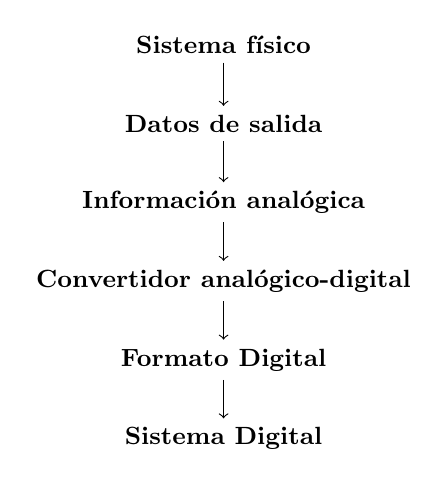
\begin{tikzpicture} 
        \small
        \node (a) at (0, 1) {\textbf{Sistema f\'{i}sico}};
        \node (b) at (0, 0) {\textbf{Datos de salida}};
        \node (c) at (0, -1) {\textbf{Informaci\'{o}n anal\'{o}gica}};
        \node (d) at (0, -2) {\textbf{Convertidor anal\'{o}gico-digital}};
        \node (e) at (0, -3) {\textbf{Formato Digital}};
        \node (f) at (0, -4) {\textbf{Sistema Digital}};

        \draw[->] (a) -- (b);
        \draw[->] (b) -- (c);
        \draw[->] (c) -- (d);
        \draw[->] (d) -- (e);
        \draw[->] (e) -- (f);
    \end{tikzpicture}
\end{center}
\medskip
\normalsize

La ventaja de usar el c\'{o}digo Gray es que la diferencia entre dos n\'{u}meros cualesquiera
es \'{u}nicamente de 1 bit.
\begin{center}
    $(Binario): (0111\,1000)$, $(Gray): (0100\,1100)$
\end{center}

Una aplicaci\'{o}n del c\'{o}digo Gray es en los datos anal\'{o}gicos se representan
mediante el cambio continuo en la posici\'{o}n de un eje.

\subsubsection*{1.7.4 C\'{o}digo ASCII}
El c\'{o}digo ASCII consta de 7-bits para su codificaci\'{o}n, por lo que tiene un conjunto
de 128 combinaciones distintas. Con $b_1 \rightarrow b_7$ siendo $b_7$ el bit m\'{a}s significativo,
por ejemplo: letra A: $100\,0001$, (columna 100, fila 0001).

Contiene 94 caracteres imprimibles y 34 caracteres no imprimibles. Estos no imprimibles son 
caracteres de control.
\begin{itemize}
    \item 26 letras min\'{u}sculas y 26 letras may\'{u}sculas. (52)
    \item 10 d\'{i}gitos decimales. (10)
    \item 32 caracteres especiales. (32)
\end{itemize}
\medbreak

\subsubsection*{1.7.5 Tipos de caracteres de control}

\begin{enumerate}
    \item \textbf{Creadores de Formato}

    Controlan la forma de imprimir, controles conocidos $\rightarrow$ m\'{a}quinas de escribir.
    \begin{itemize}
        \item (BS): Retroceso
        \item (HT): Tabulador Horizontal
        \item (CR): Retorno de carro
    \end{itemize}

    \item \textbf{Separadores de Informaci\'{o}n}

    Separan datos en divisiones como p\'{a}rrafos, l\'{i}neas, p\'{a}ginas, etc.
    \begin{itemize}
        \item (RS): Separador de Registros
        \item (FS): Separador de Archivos
    \end{itemize}

    \item \textbf{Controladores de Informaci\'{o}n}

    Transmisi\'{o}n de datos entre terminales remotas.
    \begin{itemize}
        \item (STX): Inicio de Texto
        \item (ETX): Fin de Texto
    \end{itemize}

    Encuadran un mensaje entre l\'{i}neas telef\'{o}nicas.
\end{enumerate}
(8 bits) $\rightarrow$ (1 byte) $\rightarrow$ (1 car\'{a}cter ASCII), \\
Se almacena 1 Byte por car\'{a}cter ASCII.

\subsubsection*{1.7.6 C\'{o}digo para detectar errores}

Para poder detectar errores en la comunicaci\'{o}n de datos, se agrega un bit extra.
Este bit indica la paridad:

\textbf{(Paridad):} Se refiere a la cantidad de bits 1's en un byte. Si la cantidad de
bits 1's es par, se le asigna un 0, si es impar, se le asigna un 1. Es m\'{a}s com\'{u}n
la paridad par.

\begin{verse}
    El bit de paridad se transmite, \\
    el receptor verifica la paridad del byte recibido, \\
    si la paridad es correcta, se asume que no hay error, \\
    si la paridad es incorrecta, se asume que hay un error.
\end{verse}

\subsection*{1.8 Almacenamiento Binario y Registros}

La informaci\'{o}n binaria $\rightarrow$ debe existir f\'{i}sicamente, \\
medio de almacenamiento en bits $\rightarrow$ registro, \\
un registro de $\rightarrow$ $n$ bits.
\medbreak

El estado de un registro es una tupla de $n$ bits; \\
el contenido $\rightarrow$ funci\'{o}n, la interpretaci\'{o}n $\rightarrow$ informaci\'{o}n.
\medbreak

Un registro de 16 bits:
\begin{center}
    1100001111001001
\end{center} 

Un registro puede:
\begin{itemize}
    \item \begin{center}
        \textbf{Almacenar datos} \\
        elementos discretos de informaci\'{o}n.
    \end{center}
    \item \begin{center}
        \textbf{Almacenar instrucciones} \\
        misma configuraci\'{o}n de bits, distinta interpretaci\'{o}n.
    \end{center}
\end{itemize}
\medbreak

Manipulaci\'{o}n de variables binarias $\rightarrow$ circuitos l\'{o}gicos digitales.
\medbreak
Transferencia de registros $\rightarrow$ operaci\'{o}n b\'{a}sica en sistemas digitales.
\medbreak

\subsection*{1.9 L\'{o}gica Binaria}

\begin{center}
    \textbf{Variables} $\rightarrow$ 2 valores discretos, \\
    \textbf{Operaciones} $\rightarrow$ 3 operaciones l\'{o}gicas.
\end{center}
\medbreak

\begin{flushleft}
    Se habla en t\'{e}rminos de bits, \\
    en valores de (0's y 1's), \'{a}lgebra booleana.
\end{flushleft}
\medbreak

\begin{center}
    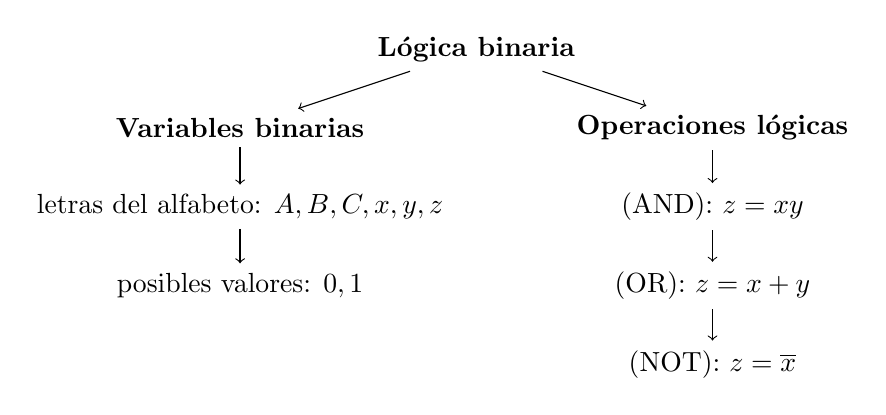
\begin{tikzpicture} 
        \node (a) at (0, 1) {\textbf{L\'{o}gica binaria}};
        \node (b) at (-3, 0) {\textbf{Variables binarias}};
        \node (c) at (3, 0) {\textbf{Operaciones l\'{o}gicas}};
        \node (d) at (-3, -1) {letras del alfabeto: $A, B, C, x, y, z$};
        \node (h) at (-3, -2) {posibles valores: $0, 1$};
        \node (e) at (3, -1) {(AND): $z = xy$};
        \node (f) at (3, -2) {(OR): $z = x + y$};
        \node (g) at (3, -3) {(NOT): $z = \overline{x}$};

        \draw[->] (a) -- (b);
        \draw[->] (a) -- (c);

        \draw[->] (b) -- (d);
        \draw[->] (d) -- (h);

        \draw[->] (c) -- (e);
        \draw[->] (e) -- (f);
        \draw[->] (f) -- (g);
    \end{tikzpicture}
\end{center}

\subsubsection*{1.9.1 Distintas interpretaciones}
\begin{flushleft}
    aritm\'{e}tica binaria: \\
    \begin{center}
        $1 + 1 = 10$
    \end{center}

    l\'{o}gica binaria: \\
    \begin{center}
        $1 + 1 = 1$
    \end{center}
\end{flushleft}

\subsubsection*{1.9.2 Compuertas l\'{o}gicas}
Son dispositivos que operan 1 o m\'{a}s entradas binarias para producir una salida binaria.

\begin{center}
    (AND), (OR), (NOT)
\end{center}

\end{document}